\documentclass[../main.tex]{subfiles}
\begin{document}
\begin{itemize}
    \item Tipi di dato non strutturati, ogni identificatore è riferito ad un \underline{unico elemento}
    \begin{itemize}
        \item \code{int}
        \item \code{float}
        \item \code{char}
    \end{itemize}
    \item Tipi di dato strutturati, mediante ogni identificatore è possibile accedere agli elementi aggregati
    \begin{itemize}
        \item \code{arrays}
        \item \code{classi}
    \end{itemize}
\end{itemize}
\textbf{Nota:} in java gli array hanno una \underline{lunghezza fissa} e possiedono elementi di un \underline{unico tipo}.

\vspace{0.5cm}
\subsection{Sintassi}
\subsubsection{Creazione}
\begin{lstlisting}[style=java]
    // Dichiarazione e creazione di un array con valori di default
    int[] voti;
    voti = new int[5];

    // In un unica riga
    int[] voti = new int[5];

    // Con inizializzazione diretta
    int[] voti = {28, 30, 25, 27, 29};
\end{lstlisting}
\textbf{Nota:} nei primi due casi l'array non viene inizializzato e di conseguenza ad ogni cella dell'array viene assenato un valore di
default, nel caso del tipo \code{int} è \code{0}.

\vspace{0.5cm}
\subsubsection{Utilizzare gli elementi}
\begin{lstlisting}[style=java]
    // Assegnare un valore ad un elemento
    voti[0] = 28;

    Assegnare un elemento di un array a una variabile
    int primoVoto = voti[0];
\end{lstlisting}

\vspace{0.5cm}
\subsubsection{Proprietà}
\begin{lstlisting}[style=java]
    // Lunghezza dell'array
    int numeroVoti = voti.length;

    // L'ultimo valore dell'array
    int ultimoVoto = voti[voti.length - 1];

    // QUESTO GENERA ERRORE DURANTE L'ESECUZIONE (NON DURANTE LA COMPILAZIONE)
    int errore = voti[voti.length];
\end{lstlisting}
\textbf{Nota:} \code{length} non è un metodo come nel caso delle stringhe quindi \underline{non vanno messe le parentesi}.

\subsection{\code{foreach}}
È possibile scorrere l'intero contenuto di un array con un ciclo \code{foreach}:
\begin{lstlisting}[style=java]
    for(int value : voti) {
        System.out.println(value);
    }
\end{lstlisting}

\vspace{0.5cm}
\subsection{Confronto}
Due array sono uguali se hanno la \underline{stessa lunghezza} e se hanno gli \underline{stessi valori nelle stesse posizioni}.

Possiamo implementare questa logica a mano o utilizzare il metodo \code{Arrays.equals}:
\begin{lstlisting}[style=java]
    import java.util.Arrays;

    System.out.println("Gli array sono uguali? " + Arrays.equals(numeri1, numeri2));
\end{lstlisting}

\vspace{0.5cm}
\subsection{Trovare massimo/minimo}
\begin{lstlisting}[style=java]
    int max = numeri[0];
    for(int i = 1; i < numeri.length; i++) {
        if(numeri[i] > max) {
            max = numeri[i];
        }
    }
\end{lstlisting}

\vspace{0.5cm}
\subsection{Aumentare la lunghezza}
\begin{lstlisting}[style=java]
    int[] valori = {1, 2, 3, 4};

    int[] tmp = new int[valori.length + 1]; 

    for(int i = 0; i < valori.length; i++)
        tmp[i] = valori[i];

    valori = tmp;
\end{lstlisting}

\pagebreak
\subsection{Gestione della memoria}
\begin{lstlisting}[style=java]
    int[] v = {3, 72, 4, 1};
    int[] w = v;

    // Cambia per entrambi gli array perchè puntano allo stesso indirizzo di memoria
    w[1] = 42;
\end{lstlisting}
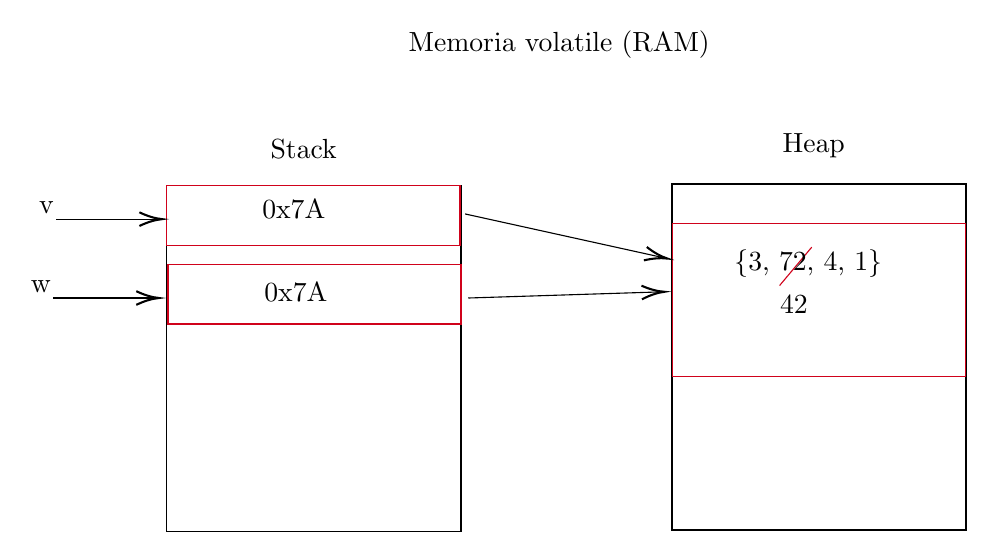
\begin{tikzpicture}[x=0.75pt,y=0.75pt,yscale=-1,xscale=1]
    %Shape: Rectangle [id:dp2878607482126624] 
    \draw   (153.33,101) -- (295,101) -- (295,267.67) -- (153.33,267.67) -- cycle ;
    %Shape: Rectangle [id:dp5159850731392541] 
    \draw   (396.67,100.33) -- (538.33,100.33) -- (538.33,267) -- (396.67,267) -- cycle ;
    %Shape: Rectangle [id:dp034822957732950965] 
    \draw  [color={rgb, 255:red, 208; green, 2; blue, 27 }  ,draw opacity=1 ] (153.33,101) -- (294.5,101) -- (294.5,129.75) -- (153.33,129.75) -- cycle ;
    %Straight Lines [id:da003920143957545252] 
    \draw    (100,117.25) -- (149,117.25) ;
    \draw [shift={(151,117.25)}, rotate = 180] [color={rgb, 255:red, 0; green, 0; blue, 0 }  ][line width=0.75]    (10.93,-3.29) .. controls (6.95,-1.4) and (3.31,-0.3) .. (0,0) .. controls (3.31,0.3) and (6.95,1.4) .. (10.93,3.29)   ;
    %Shape: Rectangle [id:dp37167315166323056] 
    \draw  [color={rgb, 255:red, 208; green, 2; blue, 27 }  ,draw opacity=1 ] (153.83,139) -- (295,139) -- (295,167.75) -- (153.83,167.75) -- cycle ;
    %Straight Lines [id:da9347723522870176] 
    \draw    (98.5,155.25) -- (147.5,155.25) ;
    \draw [shift={(149.5,155.25)}, rotate = 180] [color={rgb, 255:red, 0; green, 0; blue, 0 }  ][line width=0.75]    (10.93,-3.29) .. controls (6.95,-1.4) and (3.31,-0.3) .. (0,0) .. controls (3.31,0.3) and (6.95,1.4) .. (10.93,3.29)   ;
    %Shape: Rectangle [id:dp511806848008135] 
    \draw  [color={rgb, 255:red, 208; green, 2; blue, 27 }  ,draw opacity=1 ] (396.83,119.5) -- (538,119.5) -- (538,193.25) -- (396.83,193.25) -- cycle ;
    %Straight Lines [id:da9000176525547968] 
    \draw    (297,114.75) -- (392.55,135.82) ;
    \draw [shift={(394.5,136.25)}, rotate = 192.44] [color={rgb, 255:red, 0; green, 0; blue, 0 }  ][line width=0.75]    (10.93,-3.29) .. controls (6.95,-1.4) and (3.31,-0.3) .. (0,0) .. controls (3.31,0.3) and (6.95,1.4) .. (10.93,3.29)   ;
    %Straight Lines [id:da08015982027858559] 
    \draw    (298.5,155.25) -- (391,152.31) ;
    \draw [shift={(393,152.25)}, rotate = 178.18] [color={rgb, 255:red, 0; green, 0; blue, 0 }  ][line width=0.75]    (10.93,-3.29) .. controls (6.95,-1.4) and (3.31,-0.3) .. (0,0) .. controls (3.31,0.3) and (6.95,1.4) .. (10.93,3.29)   ;
    %Straight Lines [id:da31866551991742254] 
    \draw [color={rgb, 255:red, 208; green, 2; blue, 27 }  ,draw opacity=1 ]   (464,130.75) -- (448.5,149.25) ;
    
    % Text Node
    \draw (268.53,25.27) node [anchor=north west][inner sep=0.75pt]   [align=left] {Memoria volatile (RAM)};
    % Text Node
    \draw (202,77.67) node [anchor=north west][inner sep=0.75pt]   [align=left] {Stack};
    % Text Node
    \draw (448.67,75) node [anchor=north west][inner sep=0.75pt]   [align=left] {Heap};
    % Text Node
    \draw (90.5,107.5) node [anchor=north west][inner sep=0.75pt]   [align=left] {v};
    % Text Node
    \draw (199,146.5) node [anchor=north west][inner sep=0.75pt]   [align=left] {0x7A};
    % Text Node
    \draw (86.5,145.5) node [anchor=north west][inner sep=0.75pt]   [align=left] {w};
    % Text Node
    \draw (425.5,130.5) node [anchor=north west][inner sep=0.75pt]   [align=left] {\{3, 72, 4, 1\}};
    % Text Node
    \draw (198,106.5) node [anchor=north west][inner sep=0.75pt]   [align=left] {0x7A};
    % Text Node
    \draw (447.5,153) node [anchor=north west][inner sep=0.75pt]   [align=left] {42};
\end{tikzpicture}


\vspace{0.5cm}
\subsection{Copiare un array}
\subsubsection{Shallow copy}
\begin{itemize}
    \item Allocare la memoria necessaria
    \item Copiare valore per valore
\end{itemize}

\vspace{0.5cm}
\begin{lstlisting}[style=java]
    int[] v = {3, 72, 4, 1};
    
    int[] w = new int[v.length]

    for(int i = 0; i++ i < v.length; i++) {
        w[i] = v[i];
    }
\end{lstlisting}
che corrisponde a fare
\begin{lstlisting}[style=java]
    int[] v = {3, 72, 4, 1};
    
    int[] w = Arrays.copyOf(v, v.length);
\end{lstlisting}


\subsubsection{Deep copy}
\begin{itemize}
    \item Allocare la memoria necessaria
    \item Copiare valore per valore
    \item Se i valori degli array sono oggetti, allocare la memoria e copiare i valori ricorsivamente
\end{itemize}

\textbf{Nota:} nel caso di tipi primitivi, shallow copy e deep copy producono lo stesso risultato. Le cose cambiano se ci sono dei tipi
riferimento.


\vspace{0.5cm}
\subsection{Array multidimensionali}
\begin{itemize}
    \item Array di array
    \item Devono essere tutti dello stesso tipo
    \item Ogni riga può avere una lunghezza diversa (array frastagliati)
\end{itemize}

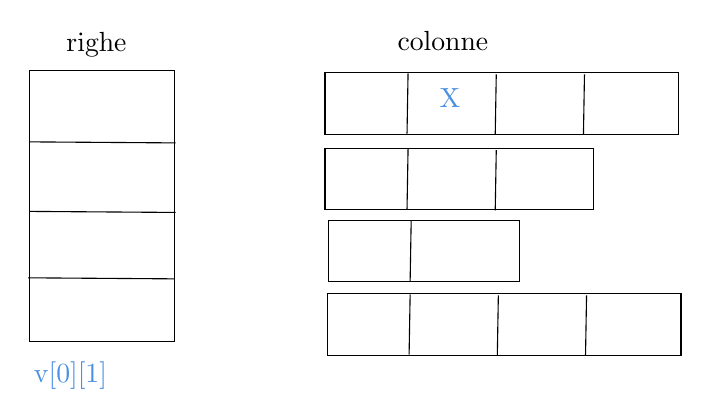
\begin{tikzpicture}[x=0.75pt,y=0.75pt,yscale=-1,xscale=1]
    %Shape: Rectangle [id:dp7152784147872497] 
    \draw   (168,50) -- (238,50) -- (238,180.25) -- (168,180.25) -- cycle ;
    %Straight Lines [id:da22373903778817406] 
    \draw    (168,84.25) -- (238.5,84.75) ;
    %Straight Lines [id:da8216526947488357] 
    \draw    (168,117.75) -- (238.5,118.25) ;
    %Straight Lines [id:da40551428764826125] 
    \draw    (167.5,149.75) -- (238,150.25) ;
    %Shape: Rectangle [id:dp020200259209480764] 
    \draw   (310.5,51) -- (481,51) -- (481,80.5) -- (310.5,80.5) -- cycle ;
    %Straight Lines [id:da714820815770691] 
    \draw    (350,80.25) -- (350.5,51.25) ;
    %Straight Lines [id:da4317115791405197] 
    \draw    (392.5,80.75) -- (393,51.75) ;
    %Straight Lines [id:da13512714855962138] 
    \draw    (435,80.75) -- (435.5,51.75) ;
    %Shape: Rectangle [id:dp25388616509385376] 
    \draw   (310.5,87.5) -- (440,87.5) -- (440,117) -- (310.5,117) -- cycle ;
    %Straight Lines [id:da716876748706907] 
    \draw    (350,116.75) -- (350.5,87.75) ;
    %Straight Lines [id:da010071016659797816] 
    \draw    (392.5,117.25) -- (393,88.25) ;
    %Shape: Rectangle [id:dp9327377227113821] 
    \draw   (312,122) -- (404,122) -- (404,151.5) -- (312,151.5) -- cycle ;
    %Straight Lines [id:da8556052749336739] 
    \draw    (351.5,151.25) -- (352,122.25) ;
    %Shape: Rectangle [id:dp18915616309979855] 
    \draw   (311.5,157.5) -- (482,157.5) -- (482,187) -- (311.5,187) -- cycle ;
    %Straight Lines [id:da6858439165484875] 
    \draw    (351,186.75) -- (351.5,157.75) ;
    %Straight Lines [id:da5289897472782741] 
    \draw    (393.5,187.25) -- (394,158.25) ;
    %Straight Lines [id:da04887338432939803] 
    \draw    (436,187.25) -- (436.5,158.25) ;
    
    % Text Node
    \draw (184.67,30) node [anchor=north west][inner sep=0.75pt]   [align=left] {righe};
    % Text Node
    \draw (344.17,29.5) node [anchor=north west][inner sep=0.75pt]   [align=left] {colonne};
    % Text Node
    \draw (364.5,57.5) node [anchor=north west][inner sep=0.75pt]  [color={rgb, 255:red, 74; green, 144; blue, 226 }  ,opacity=1 ] [align=left] {X};
    % Text Node
    \draw (169,189) node [anchor=north west][inner sep=0.75pt]   [align=left] {\textcolor[rgb]{0.29,0.56,0.89}{v[0][1]}};
\end{tikzpicture}    






\end{document}